\documentclass[tikz,border=4pt]{standalone}
\usepackage{amsmath}
\begin{document}
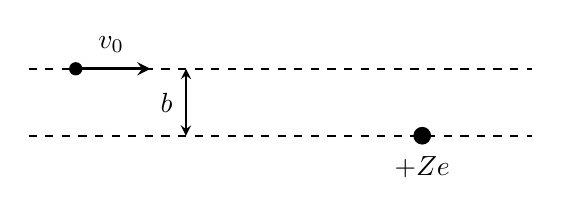
\begin{tikzpicture}[>=stealth, thick, scale=1.0]
  % Asymptotic line of incoming particle and parallel line through nucleus
  \draw[dashed, line width=0.6pt] (-3.2, 0.85) -- (3.2, 0.85);
  \draw[dashed, line width=0.6pt] (-3.2, 0) -- (3.2, 0);

  % Incoming particle and velocity arrow
  \fill (-2.6, 0.85) circle (2.4pt);
  \draw[->, line width=1.1pt] (-2.6, 0.85) -- (-1.65, 0.85);
  \node[above] at (-2.15, 0.92) {$v_0$};

  % Impact parameter b
  \draw[<->, line width=0.65pt] (-1.2, 0) -- (-1.2, 0.85);
  \node[left] at (-1.24, 0.42) {$b$};

  % Target nucleus +Ze
  \fill (1.8, 0) circle (3.2pt);
  \node[below] at (1.8, -0.14) {$+Ze$};
\end{tikzpicture}
\end{document}
